\section{The Design of Helios}

\begin{figure}[!htbp]
    \centering
    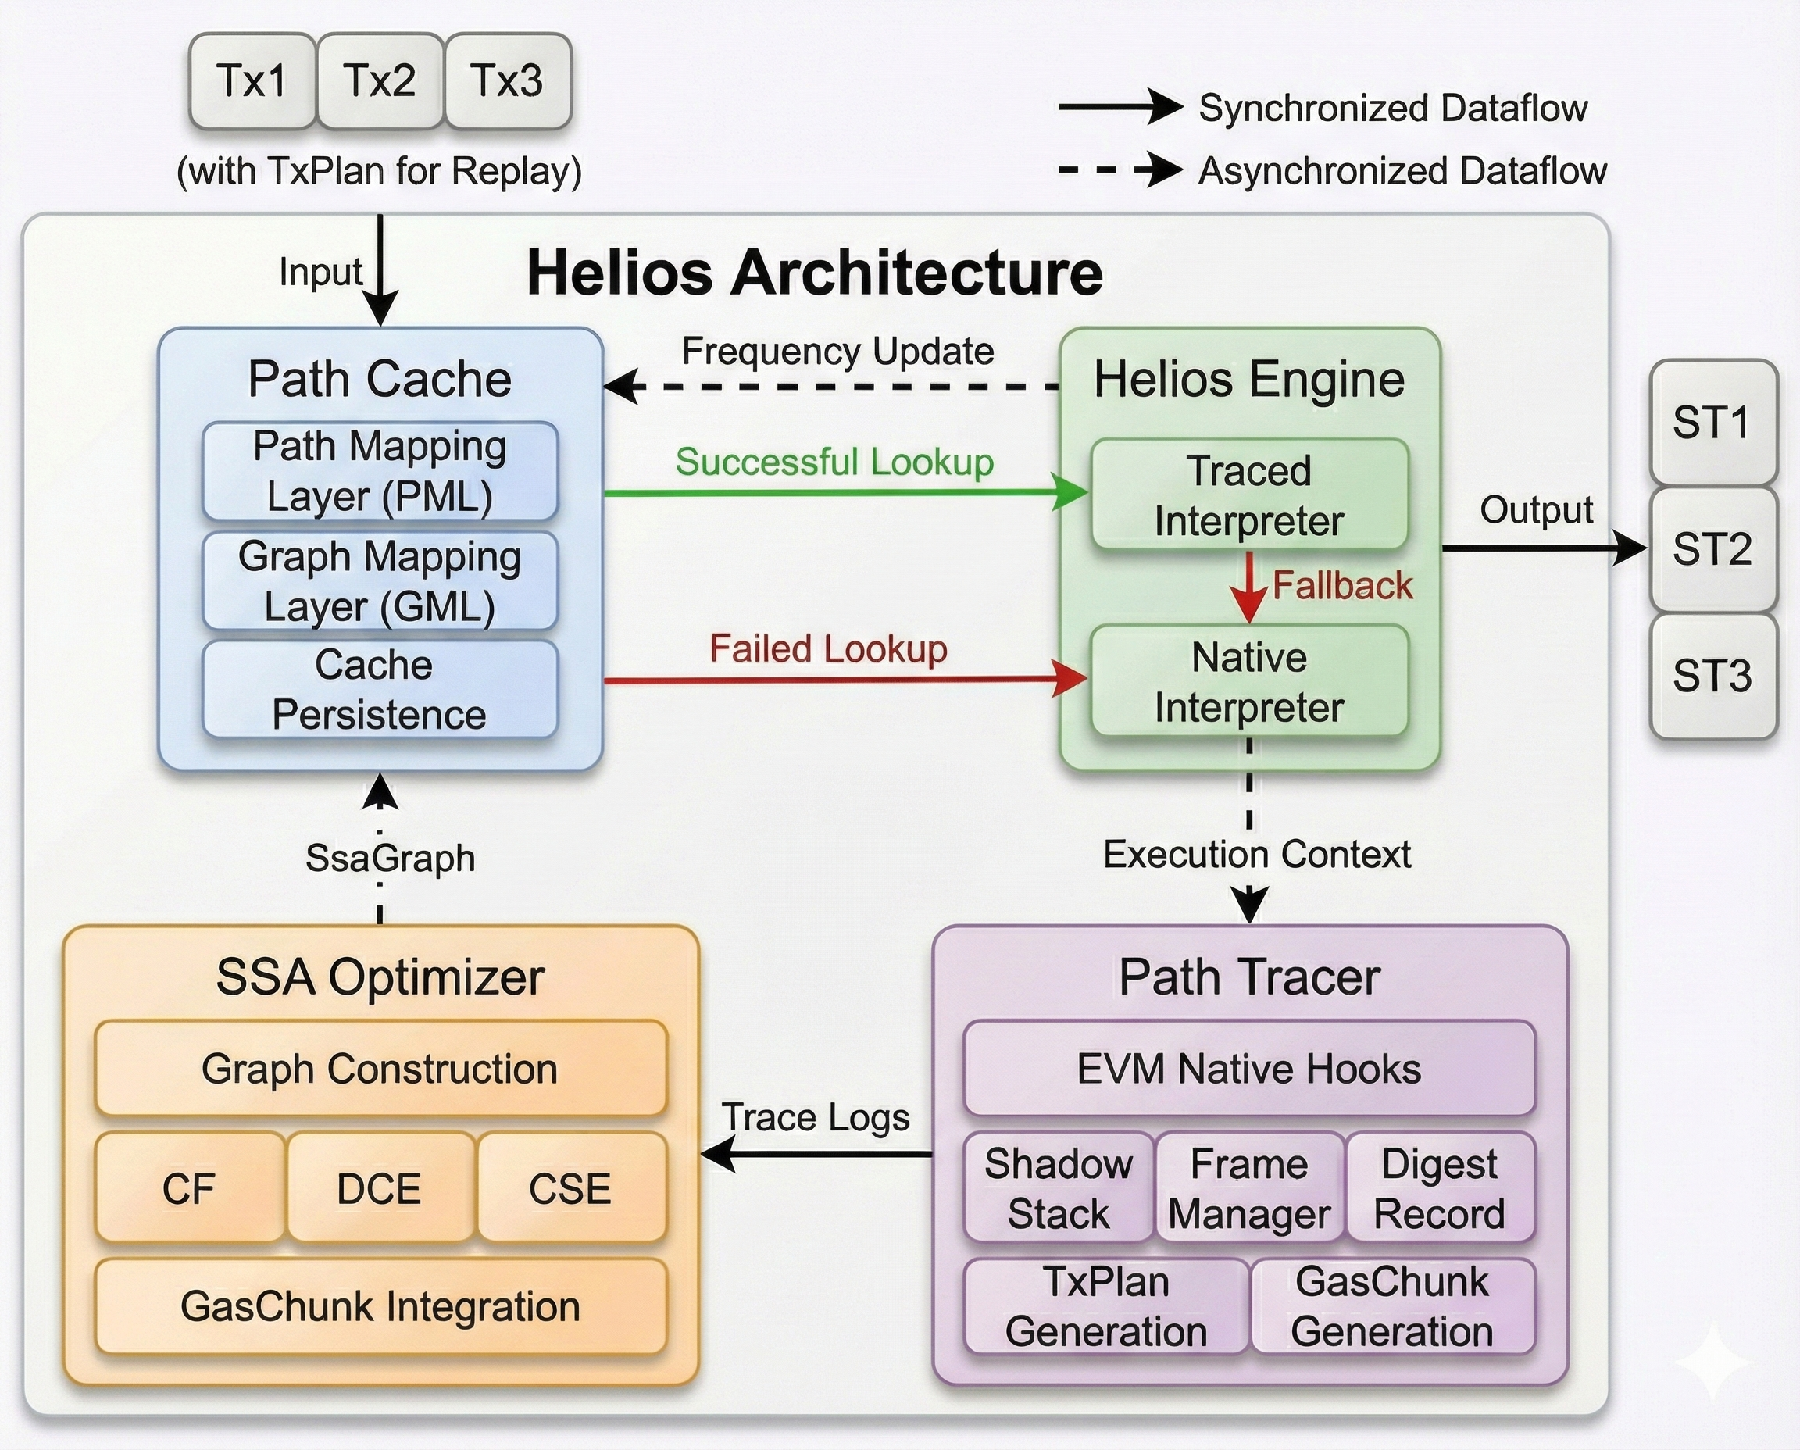
\includegraphics[width=\linewidth]{raw-figures/helios-architecture.pdf}
    \caption{Overview of the Helios architecture.}
    \label{fig:helios-architecture}
\end{figure}

\subsection{Overview}
Helios is a path-driven execution engine designed to accelerate EVM transaction processing. Its architecture is built on a continuous feedback loop that integrates four coordinated components: the Path Tracer, the SSA Optimizer, the Path Cache, and the Helios Engine. Notably, path tracing and optimization are performed asynchronously, running in parallel with the primary transaction execution flow. Figure~\ref{fig:helios-architecture} illustrates the system's high-level architecture and data flow. This asynchronous design eliminates optimization latency from the critical path, ensuring that trace generation and graph compilation do not delay transaction processing.

The system's functionality is partitioned across these four distinct components. The Path Tracer captures raw execution traces through lightweight, hook-based instrumentation of the native EVM interpreter, producing a linear execution record known as a PathLog. The SSA Optimizer transforms these PathLog entries into an SSA-like intermediate representation, termed SsaGraph, by applying a pipeline of classic compiler optimizations to eliminate redundant computations. The Path Cache serves as an in-memory memoization layer, indexing and storing optimized SsaGraph structures for rapid, low-latency retrieval. Finally, the Helios Engine orchestrates the execution of each transaction, determining whether to use a cached SsaGraph for accelerated processing or to delegate the task to the native interpreter as a fallback. 

\subsection{End-to-End Transaction Lifecycle}
The Helios architecture supports two distinct operational modes---Online and Replay---each defining a different transaction processing lifecycle. The Online mode is designed for real-time processing where execution paths are unknown, while the Replay mode is optimized for high-throughput batch processing of historical transactions with pre-determined paths. 

\subsubsection{Online Mode: Executing New Transactions}
Online mode is engineered for the real-time processing demands of full nodes and validators, where execution paths are often unknown. When a function is invoked, the Helios Engine generates an identifier based on the contract and the function being called. It uses this identifier to query the Path Cache for a corresponding SsaGraph. If a matching path is found, the Traced Interpreter begins speculative execution, validated at runtime by control-flow guards. A guard failure or a cache miss triggers an immediate, transaction-level fallback to the Native Interpreter, which executes the transaction to completion to ensure correctness.

This fallback event activates the asynchronous optimization pipeline. The Path Tracer observes the native execution and generates a detailed, linear trace of the operations performed. This trace is then dispatched to the SSA Optimizer, which transforms it into an optimized SsaGraph and its associated constant data. Finally, these new artifacts are stored in the Path Cache, populating it for subsequent executions.

\subsubsection{Replay Mode: Executing Historical Transactions}
Replay mode is tailored for the high-throughput batch processing requirements of archive nodes. In this mode, transaction execution is deterministic. Before processing, the Helios Engine retrieves a pre-computed plan for the transaction, which contains an ordered list of unique identifiers for each execution path. For each frame, the engine uses the corresponding path identifier to perform a direct lookup in the Path Cache.

This lookup is guaranteed to succeed, as the plan only references paths that were successfully traced and cached during a prior execution. The Path Cache returns the precise SsaGraph and its associated constant data. The Traced Interpreter then executes this path directly. In this mode, the speculative nature of the Online mode is entirely eliminated as there are neither cache misses nor control-flow guards needed, and the asynchronous tracing and optimization pipeline is bypassed. This streamlined process enables maximum execution throughput for reprocessing historical blocks.

\subsection{Key Data Structures}
Helios uses a set of data structures to represent, index, and orchestrate the execution of transaction paths. These abstractions manage the system's data flow, enabling both the speculative execution of Online mode and the deterministic processing of Replay mode.

\subsubsection{Path Representation}
Execution paths are captured and optimized through two primary representations:

\begin{itemize}[leftmargin=0pt, itemindent=0pt, labelwidth=1em, labelsep=0.5em]

\item \textbf{PathLog}: A raw, linear record of an execution path generated by the Path Tracer. It contains a sequence of entries, where each entry details a single operation's opcode and its stack data dependencies, recorded as references to the outputs of prior operations. The PathLog serves as the direct input to the optimization pipeline.

\item \textbf{SsaGraph}: The optimized, graph-based representation of an execution path. It is a directed acyclic graph where nodes represent operations and edges represent data dependencies. This structure makes data dependencies explicit, removing the need for a runtime stack machine and serving as the executable format for the Traced Interpreter.

\end{itemize}

\subsubsection{Path Indexing and Retrieval}
To locate and reuse SsaGraph structures, Helios employs a multi-key indexing scheme:

\begin{itemize}[leftmargin=0pt, itemindent=0pt, labelwidth=1em, labelsep=0.5em]

\item \textbf{PathDigest}: A 64-bit hash of a path's opcode sequence. It serves as a unique and compact identifier for a specific execution path. Its primary use is for deterministic lookups in the Path Cache.

\item \textbf{DataKey}: A composite key created by concatenating a contract's code hash with a PathDigest. It is used to index the constant table associated with a specific path in a specific contract instance. This key is necessary to enable a code/data separation strategy. For instance, two different ERC20 token contracts deployed from identical source code will share the same PathDigest for a transfer call. However, their bytecodes may contain different immediate values, such as those encoding the token name or total supply. The DataKey ensures that while they can reuse the same SsaGraph structure, the system retrieves the correct, contract-specific constant table for each.

\item \textbf{CallSig}: A coarse-grained identifier used for predictive path lookups in Online mode. It is generated by concatenating a contract's code hash with the 4-byte function selector from the transaction's calldata. A single CallSig can map to multiple PathDigests, each representing a distinct control-flow branch that a function invocation may follow, including both successful execution and revert paths.

\end{itemize}

\subsubsection{Execution Metadata}
Helios captures additional metadata to manage cross-frame execution and optimize performance:

\begin{itemize}[leftmargin=0pt, itemindent=0pt, labelwidth=1em, labelsep=0.5em]

\item \textbf{Transaction Plan (TxPlan)}: An ordered sequence of PathDigests that records the execution path taken by every function frame within a single transaction. TxPlans are generated during Online mode execution and indexed by block number and transaction index. In Replay mode, they provide the Helios Engine with a deterministic guide for fetching the correct SsaGraph for each frame.

\item \textbf{GasChunk}: A pre-computed value representing the cumulative static gas cost of a sequence of operations. This sequence is defined as the set of instructions occurring between two specific, pre-defined opcodes that interact with the gas counter. This metadata is attached to the SsaGraph and allows the Traced Interpreter to perform a single, bulk gas deduction instead of per-instruction accounting, reducing overhead while maintaining gas-semantic equivalence.

\end{itemize}

\subsection{Component Design and Implementation}
This section details the internal design and mechanisms of each of Helios's four primary components. It describes how each component fulfills its role in the end-to-end transaction lifecycle, transforming its inputs into the data structures required by the next stage of the pipeline.


\begin{algorithm}[!htbp]
\small
\caption{Shadow Stack Tracing}
\label{alg:shadow-stack-tracing}
\KwIn{$op$: Current EVM opcode}
\KwIn{$S_{evm}$: EVM value stack (after opcode execution)}
\KwIn{$S_{\ell}$: Shadow stack of LSNs tracking value provenance}
\KwOut{$e$: Trace log entry containing the opcode, current LSN, input dependencies, and output value}
\KwOut{Updated $S_{\ell}$}

\tcp{Extract input dependencies from shadow stack}
$D_{in} \gets []$ \\
$k \gets$ \textsc{GetInputCount}$(op)$ \\
\For{$i \gets 1$ \KwTo $k$}{
    $\ell \gets S_{\ell}$.\textsc{Pop}() \\
    $D_{in}$.\textsc{Append}$(\ell)$ \\
}

\tcp{Record output value and assign new LSN}
\eIf{$op$ produces stack output}{
    $v_{out} \gets S_{evm}$.\textsc{Top}() \\
    $\ell_{curr} \gets$ \textsc{NextLSN}() \\
    $S_{\ell}$.\textsc{Push}$(\ell_{curr})$ \\
}{
    $v_{out} \gets \bot$ \tcp*{No output, e.g., POP, JUMP}
    $\ell_{curr} \gets$ \textsc{NextLSN}() \\
}

\tcp{Handle stack manipulation instructions}
\If{$op \in \{\text{\texttt{DUP1}}, \text{\texttt{DUP2}}, \ldots, \text{\texttt{DUP16}}\}$}{
    $d \gets op - \text{\texttt{DUP1}} + 1$ \\
    $\ell_t \gets S_{\ell}[d]$ \tcp*{Peek without pop}
    $S_{\ell}$.\textsc{Push}$(\ell_t)$ \tcp*{Duplicate LSN}
}
\If{$op \in \{\text{\texttt{SWAP1}}, \text{\texttt{SWAP2}}, \ldots, \text{\texttt{SWAP16}}\}$}{
    $d \gets op - \text{\texttt{SWAP1}} + 1$ \\
    $S_{\ell}$.\textsc{Swap}$(0, d)$ \tcp*{Swap LSNs}
}

\tcp{Create log entry}
$e \gets \langle op, \ell_{curr}, D_{in}, v_{out} \rangle$ \\

\Return{$e$}

\end{algorithm}

\subsubsection{Path Tracer: Lightweight Execution Path Tracing}
The Path Tracer is the system's instrumentation component, responsible for observing native EVM execution and producing the raw PathLog data structure alongside TxPlan and GasChunk.

\noindent\textbf{Instrumentation Mechanism.} Path Tracer implements non-invasive instrumentation via the EVM's Hook interface, subscribing to six event types: \texttt{step} and \texttt{step\_end} for opcode-level observation, \texttt{call} and \texttt{call\_end} for external invocations, and \texttt{create} and \texttt{create\_end} for contract deployment. This hook-based design decouples the tracer from the interpreter, enabling passive observation without modifying execution semantics.

To capture stack data dependencies, the tracer employs a shadow stack. This shadow stack mirrors the EVM's value stack but stores 32-bit Log Sequence Numbers (LSNs) instead of 256-bit values. Each LSN uniquely identifies the operation that produced the corresponding value on the EVM stack.

The tracing process, detailed in Algorithm~\ref{alg:shadow-stack-tracing}, is driven by the step\_end hook, which fires after each opcode execution. For a given opcode, the algorithm first determines the number of required inputs and pops the corresponding LSNs from the shadow stack to form the dependency list. Next, a new LSN is assigned to the current operation. If the operation produces a stack output, this new LSN is pushed onto the shadow stack, tracking the provenance of the new value. Crucially, for stack manipulation opcodes like DUP and SWAP that do not create new values but reorder existing ones, the algorithm mirrors these structural changes on the shadow stack to maintain a one-to-one correspondence with the EVM's value stack. This process ensures that the generated PathLog entry correctly links each operation to the LSNs of its true data dependencies.

\noindent\textbf{Metadata Generation.} The Path Tracer is also responsible for generating two key metadata structures: GasChunk and TxPlan. To generate GasChunk metadata, the tracer identifies a set of six gas delimiter opcodes, namely GAS, RETURN, STOP, REVERT, CREATE, and CREATE2. The tracer accumulates the static gas costs of all operations executed between two consecutive delimiters. Upon encountering a delimiter, it finalizes a GasChunk entry containing the accumulated cost. If an execution path terminates without an explicit delimiter, a synthetic STOP is considered to ensure all paths are properly chunked.

The TxPlan for a transaction is constructed using a placeholder mechanism. When a new frame is entered via the call or create hook, a placeholder is appended to the current TxPlan. When the frame execution completes via the call\_end or create\_end hook, the final, computed PathDigest for that frame replaces the placeholder. This ensures the TxPlan accurately reflects the final sequence of executed paths.

\noindent\textbf{Path Validation and Filtering.} To ensure that system resources are spent only on reusable paths, the tracer performs a health check. During the call\_end hook, it inspects the frame's exit status. Paths that terminate due to VM-level exceptional conditions, specifically out-of-gas errors, are discarded. In contrast, deterministic application-level terminations, including both successful returns and REVERT operations, are retained and cached. This distinction is critical because REVERT paths represent reproducible control-flow branches such as failed require checks or insufficient balance validations, which exhibit high reusability across transactions. VM-level exceptions like OOG, however, exhibit low reusability, as an OOG exception may manifest at any opcode depending on the transaction's gas limit. Recording all possible OOG points would induce exponential path explosion. For a sequence of $n$ opcodes, tracking every potential OOG point generates $O(n)$ distinct failure paths, fragmenting the cache without improving hit rates for deterministic execution. Consequently, only deterministically terminated paths, whether successful or reverted, are formatted into PathLog entries and forwarded to the SSA Optimizer.

\subsubsection{SSA Optimizer: Graph Construction and Optimization}
The SSA Optimizer is a pure-function component that transforms a raw PathLog from the Path Tracer into an optimized SsaGraph and an associated constant table. This process involves four distinct stages.

\noindent\textbf{Graph Construction.} The optimizer first constructs an initial SsaGraph from the input PathLog. Each entry in the PathLog's sequence is converted into a corresponding node in the graph. Directed edges are then created to represent data dependencies by connecting each node to the predecessor nodes indicated in its $D_{in}$ LSN list. The result is a direct graph-based representation of the linear trace. 

\noindent\textbf{Three-Stage Optimization Pipeline.} The initial graph then undergoes a three-stage optimization pipeline to eliminate computational redundancy: Constant Folding, Dead Code Elimination, and Common Subexpression Elimination. This specific ordering exploits cascading optimization opportunities whereby constant propagation exposes previously unreachable dead code, and the subsequent elimination of dead operations narrows the search space for common subexpression detection.

\begin{itemize}[leftmargin=0pt, itemindent=0pt, labelwidth=1em, labelsep=0.5em]

\item \textbf{Constant Folding.} The first pass identifies all nodes corresponding to PUSH instructions. Their immediate values are extracted and placed into a constant table. The optimizer then iteratively propagates these constants through subsequent nodes that have no observable side effects, specifically operations that do not modify memory, storage, or system state. Nodes whose computations are fully resolved at compile time are marked as REMOVED, and their outputs are added to the constant table.

\item \textbf{Dead Code Elimination.} The second pass performs a backward dataflow analysis, starting from nodes that have observable side effects. Any node whose output is not consumed by a non-removed successor is also marked as REMOVED. This process repeats until a fixed point is reached, ensuring that all computationally unnecessary operations are pruned from the graph.

\item \textbf{Common Subexpression Elimination.} The final pass identifies and merges redundant computations. To do this, it constructs a unique computational fingerprint for each side-effect-free operation. This fingerprint is a deterministic value derived from the operation's opcode and the LSNs of its input nodes. Formally, an operation with opcode $o$ consuming inputs from nodes with LSNs $\ell_i$ and $\ell_j$ yields the fingerprint $\langle o, i, j \rangle$. For example, an \texttt{ADD} operation with inputs $\ell_5$ and $\ell_{12}$ produces the fingerprint $\langle \texttt{ADD}, 5, 12 \rangle$. Nodes that share an identical fingerprint are considered redundant and are unified, with all consuming nodes redirected to reference the first canonical occurrence.

\end{itemize}

\noindent\textbf{GasChunk Integration.} Following the optimization pipeline, the optimizer integrates the GasChunk metadata collected by the Path Tracer. It retrieves the list of GasChunks from the PathLog and attaches each pre-computed gas cost to its corresponding delimiter node within the SsaGraph. This annotation embeds the gas accounting information directly into the executable graph structure.

\noindent\textbf{Graph Compaction and Output.} In the final stage, the optimizer physically deletes all nodes previously marked as REMOVED to produce a compact graph. It finalizes the constant table, containing all immediate values and folded constants from the optimization phase. The resulting SsaGraph, its constant table, and associated identifiers are then transmitted to the Path Cache for storage.

\subsubsection{Path Cache: Execution Path Memoization}
To efficiently support both the probabilistic lookups of Online mode and the deterministic lookups of Replay mode, the Path Cache employs a two-tier architecture that separates prediction logic from canonical storage.

\begin{itemize}[leftmargin=0pt, itemindent=0pt, labelwidth=1em, labelsep=0.5em]

\item \textbf{Path Mapping Layer (PML)}: A frequency-based prediction index that supports Online mode's speculative execution. For each CallSig, it maintains a dual-index structure consisting of a frequency map for O(1) frequency queries and a sorted index for O(log k) maximum frequency retrieval, where k denotes the number of distinct frequency values. The PML returns the unique PathDigest with maximum access count for a given CallSig. If multiple paths share the maximum frequency, the lookup returns no prediction, prioritizing prediction accuracy over coverage as low-confidence speculation would incur guard validation overhead.

\item \textbf{Graph Mapping Layer (GML)}: A deterministic key-value store that serves as the canonical repository for all optimized execution artifacts. It implements the code/data separation strategy through two distinct mappings. The first maps each PathDigest to its corresponding SsaGraph structure, enabling code reuse across contracts with identical bytecode structure. The second maps each DataKey to a contract-specific constant table, ensuring correct constant retrieval for contracts that share code but differ in embedded immediate values.

\end{itemize}

\include{algorithm/online_lookup}

\noindent\textbf{Query Protocols.} The cache's query protocol differs based on the operational mode. In Online mode, a query begins at the PML. The engine provides a CallSig, and the PML retrieves the sorted index for that CallSig under a read lock. It inspects the highest frequency set and returns the associated PathDigest only if it is unique; if multiple paths share the maximum frequency, the query returns no prediction. When a prediction succeeds, the PathDigest is combined with the contract's code hash to form a DataKey, which is then used to query the GML for the SsaGraph and its corresponding constant table. The PathDigest is also returned to the engine for use in the subsequent feedback loop. The complete lookup process is detailed in Algorithm~\ref{alg:online-lookup}.

In contrast, Replay mode bypasses the PML entirely. The engine provides a PathDigest retrieved from a TxPlan and a DataKey. These keys are used to perform a direct, deterministic lookup in the GML to retrieve the SsaGraph and its constant table. For any path referenced in a TxPlan, this lookup is guaranteed to succeed.

\noindent\textbf{Update and Persistence.} The cache's update protocol distinguishes between two types of events, each serving a different purpose in maintaining the cache's accuracy and coverage. The first type occurs when the SSA Optimizer generates a new SsaGraph, triggering a comprehensive update. The new graph and its constant table are stored in the GML, while the PML initializes or updates the frequency statistics for the corresponding CallSig-PathDigest pair. This mechanism serves as the primary method for populating the cache with new content discovered during native execution.

The second type of update is triggered when the Helios Engine successfully completes a transaction using a cached SsaGraph in Online mode. This event initiates a lightweight feedback update in which the engine signals the PML to increment the access counter for the specific PathDigest that was executed. The PML acquires a write lock on the corresponding frequency statistics and performs an atomic update in O(log k) time: it removes the PathDigest from its old frequency set in the sorted index, increments its frequency in the frequency map, and inserts it into the new frequency set. This feedback loop reinforces the dominance of successful and frequently executed paths, directly improving the accuracy of future predictions. The complete update protocol is formalized in Algorithm~\ref{alg:path-frequency-update}.

Because the Path Tracer and SSA Optimizer execute asynchronously relative to the Helios Engine, PML operations are protected by fine-grained read-write locks on a per-CallSig basis to ensure thread safety while maximizing concurrency. Read operations, such as hot path prediction, allow concurrent access, while write operations, such as frequency updates, acquire exclusive locks for bounded time.

\noindent\textbf{Checkpoint generation and cleanup.} To ensure durability and enable fast node restarts, the system generates checkpoints every N blocks, serializing the cache's contents to disk. The default policy preserves all cached paths, but a pruning mechanism based on CallSig access frequency is provided. The access threshold can be configured to evict CallSigs, along with their associated graphs and data, falling below the specified frequency, trading coverage for storage efficiency.

\noindent\textbf{Recovery and bootstrapping.} Upon node restart, the Path Cache loads verified high-value paths from checkpoints, immediately achieving high prediction accuracy without a cold-start learning phase. The sorted indices are reconstructed in O(N log k) time during deserialization, where N is the total number of unique paths. The loaded paths represent optimized hotspots from historical execution, validated through frequency and predictability metrics. For paths absent from checkpoints, the system employs lazy regeneration, tracing and optimizing them on-demand during execution to gradually expand path coverage.

\subsubsection{Helios Engine: Dual-Mode Execution Orchestrator}
The Helios Engine is the central orchestrator that coordinates transaction processing. It integrates with the host EVM implementation by replacing its per-frame execution loop while inheriting its mature state and memory management infrastructure. For instance, in its integration with Revm, Helios leverages the host's high-performance memory subsystem, which amortizes allocation overhead by partitioning a pre-allocated byte array across multiple frames via logical checkpointing. Similarly, it inherits Revm's optimized storage access model, which uses in-memory caching and prewarming to avoid redundant disk lookups and a transaction-local journal to buffer state changes for atomic commits. By building upon this robust foundation for state handling, the Helios Engine can focus its design exclusively on optimizing the computational flow within each execution frame. It assumes full control over how opcodes are interpreted, selecting between its two internal interpreters---the Traced Interpreter and the Native Interpreter---based on the operational mode and cache state.

\noindent\textbf{Transaction-Scoped Execution Model.} A core design principle of the engine is its transaction-scoped execution model. All execution attempts, whether using the Traced Interpreter or the Native Interpreter, operate at the granularity of a full transaction. If any failure occurs during a traced execution---such as a cache miss, a guard violation, or an out-of-gas condition---the engine discards all partial work for that transaction and restarts its execution from the beginning using the Native Interpreter. This strategy eliminates the need for complex, fine-grained state checkpointing or rollback mechanisms, leveraging the EVM's inherent transaction-level atomicity to ensure correctness.

\include{algorithm/traced-execution}

\noindent\textbf{The Traced Interpreter.} When the Path Cache returns a valid SsaGraph, the engine dispatches execution to the Traced Interpreter. Its execution loop, formally detailed in Algorithm~\ref{alg:traced-execution}, is designed for high-speed graph processing and differs from a standard EVM interpreter in three key aspects.

First, it replaces the EVM's stack machine with a register-based model. As shown in the algorithm, a virtual register file is allocated, and each SsaGraph node's result is stored at an index corresponding to its LSN. An operation's inputs are sourced directly from this array, eliminating all stack manipulation overhead.

Second, in Online mode, it enforces speculative execution guards. The algorithm demonstrates how, before executing a JUMP or JUMPI, the interpreter computes the runtime jump target and validates it against the statically cached target from the SsaGraph. Any mismatch triggers an immediate transaction-level fallback. These guards are disabled in Replay mode.

Third, it implements chunked gas accounting, distinguishing between static and dynamic gas costs. For most instructions, no check is performed. At delimiter nodes, the cumulative static cost from the GasChunk is deducted in a single operation. Any instruction with dynamic gas costs such as memory expansion triggers a separate, per-instruction calculation and deduction. This hybrid approach maintains exact gas-semantic equivalence while minimizing verification overhead.

\subsection{Security Considerations}

Beyond the JIT Bomb resistance established through the path-driven paradigm in \S\ref{sec:path-vs-contract}, Helios's design inherently mitigates path explosion attacks. An adversary might attempt to degrade system performance by constructing malicious contracts that generate millions of unique execution paths for a single function signature, potentially flooding the cache and consuming optimization resources.

Helios's architecture naturally defends against this attack vector through three complementary mechanisms. The frequency-based Path Mapping Layer ensures that only paths with demonstrated reusability are predicted and accelerated. Attack-generated paths remain perpetually classified as cold paths due to low execution counts, excluded from the prediction model. The checkpoint pruning mechanism evicts CallSigs with access frequencies below a configurable threshold, preventing malicious cold paths from consuming long-term storage while retaining legitimate hot paths. The transaction-scoped execution model ensures that cache misses simply trigger fallback to the Native Interpreter, maintaining correctness and baseline performance for unpredicted paths.

Consequently, path explosion attacks impose only bounded costs on asynchronous tracing and temporary cache occupancy without degrading performance for legitimate transactions. This robustness emerges naturally from the frequency-based filtering and bounded resource allocation inherent to Helios's design.

